\q{16}{Knowledge versus Participation}
\vskip .2 in
Berkeley is an interdisciplinary place! A rhetoric professor has been collecting data on students' use of social media to discuss current events, and decides to combine her data with the political scientist's data in the previous question. The data are not anonymous, so the professors are able to link student's current events knowledge scores to a "participation factor" (a continuous value from 0 to 10) that assesses how often students engage with political causes online. 
The following is a scatter plot of the current events knowledge scores  (from question 5) versus the participation factor. 
\begin{center}
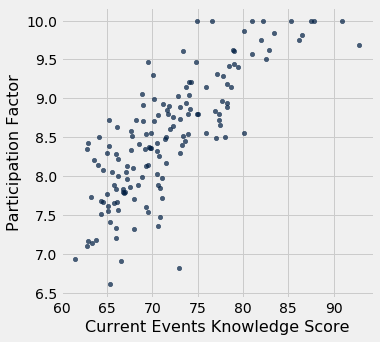
\includegraphics[scale=.8]{figures/regression_scatter.png}
\end{center}
Here is some summary information about the data:
\begin{itemize}
    \item The average current events knowledge score is 71.7, and the standard deviation of the current events knowledge score is 6.2. 
    \item The average participation factor was 8.5, and the standard deviation of the participation factor is 0.78.
    \item The correlation coefficient between current events knowledge and the participation factor across the 150 students is 0.8.
\end{itemize}

\begin{enumerate}
\subq{2} What is the slope of the least squares regression line predicting participation factor from current events knowledge score? Do not simplify your answer (show your work!).\\
\solution{$0.8 \times \frac{0.78}{6.2}$}
\vskip 0.5in
\subq{2} What is the intercept of the least squares regression line predicting participation factor from current events knowledge score? Do not simplify your answer (show your work!).\\
\solution{$8.5 - (0.8 \times \frac{0.78}{6.2})\times 71.7$}
\clearpage
\subq{6} The rhetoric professor plotted three lines on the scatter plot. They then plotted the errors between these lines and the data. \textbf{Match the three lines (A, B, C) to their corresponding error plots.} One error plot does not have a matching line.
\vskip 0.1in

\begin{center}
    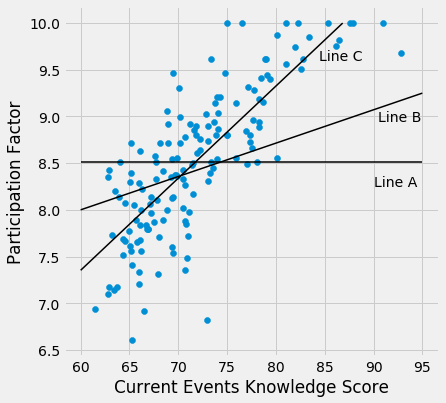
\includegraphics[scale=.42]{figures/regression_lines.png}
    \\[8pt]
    \textbf{Pick one of the bubbles for each of the following error plots.}
\end{center}
\vskip 0.1in
\begin{tabular}{l@{\hskip 0.8in}l@{\hskip 0.1in}l@{\hskip 0.1in}l}
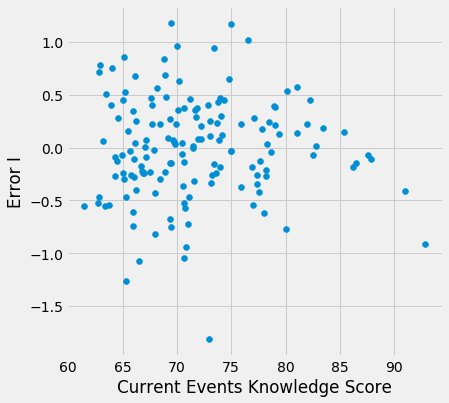
\includegraphics[scale=.41]{figures/residuals.png}
&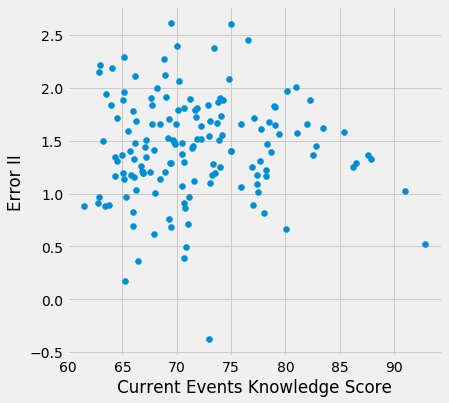
\includegraphics[scale=.41]{figures/wrong_error_b.png}
\\[2pt]
%solutions for first two plots
\begin{tabular}{l@{\hskip 0.5in}l@{\hskip 0.1in}l@{\hskip 0.1in}l}
&\bubble Line A{\hskip 0.1in}&\bubble Line B{\hskip 0.1in}\\ &\solutionbubble Line C{\hskip 0.1in}&\bubble No match
\end{tabular}
&\begin{tabular}{l@{\hskip 0.5in}l@{\hskip 0.1in}l@{\hskip 0.1in}l}
&\bubble Line A{\hskip 0.1in}&\bubble Line B{\hskip 0.1in}\\ &\bubble Line C{\hskip 0.1in}&\solutionbubble No match
\end{tabular}\\[18pt]

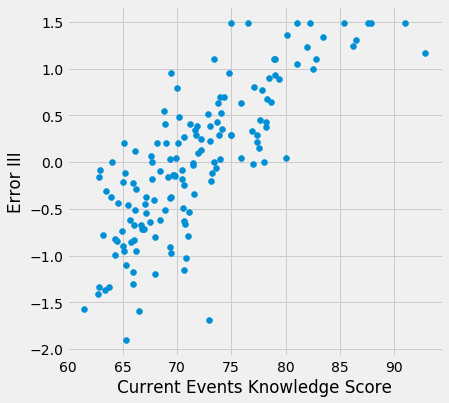
\includegraphics[scale=.41]{figures/error_from_average.png}
&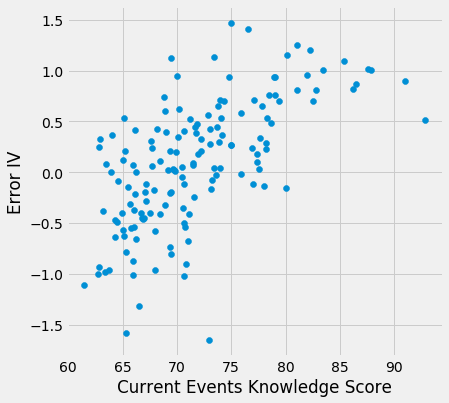
\includegraphics[scale=.41]{figures/error_from_bad_line.png}\\[2pt]

%solutions for second two plots
\begin{tabular}{l@{\hskip 0.5in}l@{\hskip 0.1in}l@{\hskip 0.1in}l}
&\solutionbubble Line A{\hskip 0.1in}&\bubble Line B{\hskip 0.1in}\\ &\bubble Line C{\hskip 0.1in}&\bubble No match
\end{tabular}
&\begin{tabular}{l@{\hskip 0.5in}l@{\hskip 0.1in}l@{\hskip 0.1in}l}
&\bubble Line A{\hskip 0.1in}&\solutionbubble Line B{\hskip 0.1in}\\ &\bubble Line C{\hskip 0.1in}&\bubble No match
\end{tabular}
\end{tabular}


\vskip 0.2in
\subq{2} One of the three lines in the plot in part \textbf{c} is the least squares regression line, and one line is the line \textit{predicted y = average(y)}. Which one is which? 
\vskip 0.1in
\begin{center}
\textbf{Least Squares Regression Line}
\vskip 0.1in
\begin{tabular}{l@{\hskip 0.3in}l@{\hskip 0.3in}l@{\hskip 0.3in}l}
\bubble Line A
&\bubble Line B
&\solutionbubble Line C
\end{tabular}
\vskip 0.2in
\textbf{\textit{predicted y = average(y)}}
\vskip 0.1in
\begin{tabular}{l@{\hskip 0.3in}l@{\hskip 0.3in}l@{\hskip 0.3in}l}
\solutionbubble Line A
&\bubble Line B
&\bubble Line C
\end{tabular}
\end{center}
\vskip 0.25in
\subq{1} Rank the mean squared error of the three lines from smallest to largest:
\vskip 0.1in
\begin{tabular}{l@{\hskip 0.5in}l@{\hskip 0.5in}l@{\hskip 0.5in}l}
\bubble A, B, C
&\bubble B, C, A
&\bubble A, C, B\\[6pt]
\bubble B, A, C
&\bubble C, A, B
&\solutionbubble C, B, A

\end{tabular}
\vskip 0.25in
\subq{3} Select \textbf{all} true statements we can justifiably conclude. If you do not have enough information to evaluate whether the statement is true or false, DO NOT select it.
\vskip 0.1in
\solutionbox The root mean squared error (RMSE) of line A is equal to the standard deviation of the participation score.
\vskip 0.1in
\checkbox The root mean squared error of line B is equal to the standard deviation of the fitted values from line B.
\vskip 0.1in
\solutionbox The root mean squared error of line C is equal to the standard deviation of the residuals. 
\vskip 0.1in
\solutionbox It is impossible to create a linear model that will give you a smaller root mean squared error than the root mean squared error from line C.

\end{enumerate}